%&LaTeX
% !TEX encoding = UTF-8 Unicode
\documentclass{report}
\usepackage[utf8]{inputenc}
\usepackage[T1]{fontenc}
\usepackage{textcomp}
\usepackage{float,fancyvrb}
\usepackage{listings}

%\usepackage{graphicx}
\usepackage{longtable}
\usepackage{color}

\usepackage{ifpdf}

\ifx\pdftexversion\undefined %if using TeX
    \usepackage{graphicx}
\else %if using PDFTeX
    \ifpdf %if using PDFTeX in PDF mode
        \usepackage[pdftex]{graphicx}
        \DeclareGraphicsExtensions{.pdf,.png,.mps}
        \usepackage{pgf}
    \else %if using TeX or PDFTeX in TeX mode
        \usepackage{graphicx}
        \DeclareGraphicsExtensions{.eps,.bmp}
        \DeclareGraphicsRule{.emf}{bmp}{}{}% declare EMF filename extension
        \DeclareGraphicsRule{.png}{bmp}{}{}% declare PNG filename extension
        \usepackage{pgf}
        \usepackage{pstricks} %variant: \usepackage{pst-all}
\fi

%\setlength{\paperheight}{297mm}
%\setlength{\paperwidth}{210mm}
%\setlength{\voffset}{11mm}
\setlength{\topmargin}{0mm}
\setlength{\headsep}{0mm}
\setlength{\headheight}{0mm}
\setlength{\textheight}{235mm}
\setlength{\hoffset}{-4mm}
\setlength{\textwidth}{166mm}
\setlength{\oddsidemargin}{0mm}
\setlength{\evensidemargin}{0mm}
\setlength{\marginparwidth}{0mm}
\setlength{\marginparpush}{0mm}
%\setlength{\columnsep}{6mm}
%\setlength{\parindent}{0mm}


\definecolor{color01}{rgb}{0.00,0.00,0.00}
\definecolor{color02}{rgb}{0.00,0.00,1.00}
\definecolor{color06}{rgb}{1.00,0.00,0.00}
\definecolor{color08}{rgb}{1.00,1.00,1.00}
\definecolor{color17}{rgb}{0.14,0.25,0.38}
\definecolor{color20}{rgb}{0.31,0.51,0.74}
\definecolor{color26}{rgb}{0.50,0.50,0.50}

%% Added by Jong -- to enable \subsubsection
\setcounter{secnumdepth}{3}
\usepackage{hyperref}

\newcommand{\comment}[1]{}
\newcommand{\adiosversion}{ADIOS 1.6\xspace}

%%%%%%%%%%%%%%%%%%%%%%%%%%%%%%%%%%%%%%%%%%%%%%%%%%%%%%%%%%%%%%%%%%%%%%%
% Define syntax highlighting for ADIOS
\lstdefinelanguage{ADIOS}
{
sensitive=true,
keywordsprefix=ADIOS_,
morekeywords=[1]{
adios_errno, err_file_not_found, err_end_of_stream, err_step_notready, err_step_deleted},
morekeywords=[2]{
% Write API (XML)
adios_init, adios_finalize, adios_open, adios_write, adios_read, adios_close, 
adios_group_size, adios_set_path_var, adios_set_path, 
adios_end_iteration, adios_start_calculation, adios_stop_calculation,
% Write API (Non-XML)
adios_init_noxml, adios_declare_group, adios_free_group, adios_define_var, 
adios_define_attribute, adios_allocate_buffer, adios_select_method,
adios_get_write_buffer,
% Read API (1.4)
adios_read_init_method, adios_read_finalize_method,
adios_read_open_file, adios_read_open, adios_read_close,
adios_inq_var, adios_inq_var_byid, adios_free_varinfo,
adios_inq_var_stat, adios_inq_var_blockinfo,
adios_get_attr, adios_get_attr_byid,
adios_schedule_read, adios_schedule_read_byid, adios_perform_reads, adios_check_reads,
adios_advance_step, adios_release_step,adios_free_chunk,
adios_selection_boundingbox, adios_selection_points, adios_selection_writeblock, 
adios_selection_delete, adios_selection_auto, adios_errmsg,
adios_type_to_string, adios_type_size, adios_get_grouplist,
% Fortran Read
adios_reset_dimension_order, adios_inq_ngroups, adios_inq_groupnames, 
adios_group_view, adios_inq_file, adios_inq_varnames, adios_inq_attrnames,
adios_inq_attr, adios_get_scalar, adios_get_statistics},
morecomment=[l]{//},morecomment=[s]{/*}{*/},
morestring=[b]",morestring=[b]',
}

\lstdefinelanguage{cython}[]{python}
{
sensitive=true,
keywordsprefix=ADIOS_,
keywords={def, cpdef, cdef, public, class, self},
morekeywords=[1]{
int64_t, uint64_t, int, long, float, double, char, bytes, tuple, list, dict},
upquote=true,
}

\lstdefinelanguage{ADIOS-python}[]{python}
{
upquote=true,
}

\definecolor{gray}{rgb}{0.35,0.35,0.35}
\definecolor{gray85}{rgb}{0.85,0.85,0.85}
\definecolor{javared}{rgb}{0.6,0,0}
\definecolor{javagreen}{rgb}{0.25,0.5,0.35}
\definecolor{javapurple}{rgb}{0.5,0,0.35}
\definecolor{javadocblue}{rgb}{0.25,0.35,0.75}

\lstset{language=ADIOS, basicstyle=\ttfamily, numbers=none,
  showspaces=false, showstringspaces=false,
  keywordstyle=[1]\color{javapurple},
  keywordstyle=[2]\color{blue}\bf,
  stringstyle=\color{javared},
  commentstyle=\color{javagreen},
  captionpos=b,
  frame=no,
  escapechar=`,
}
% End of syntax highlight def for ADIOS
%%%%%%%%%%%%%%%%%%%%%%%%%%%%%%%%%%%%%%%%%%%%%%%%%%%%%%%%%%%%%%%%%%%%%%%

\begin{document}


\vspace{24pt}
\begin{flushright}
{\color{color08} \textbf{ORNL/TM-2009/100\label{OLEHLINK6}}}
\end{flushright}

\vspace{60pt}
{\huge \textbf{ADIOS 1.5.0 Developer's Manual}}

\vspace{36pt}
\textbf{July 2012\pagebreak{}}


\begin{longtable}{|p{4.443in}|p{0.057in}|}
\hline

\begin{center}
{\small \textbf{DOCUMENT AVAILABILITY}}
\end{center}


{\small Reports produced after January 1, 1996, are generally available free via 
the U.S. Department of Energy (DOE) Information Bridge:}


\leftskip=18pt
{\small \textbf{Web site:}}{\small  http://www.osti.gov/bridge}


\leftskip=0pt
{\small Reports produced before January 1, 1996, may be purchased by members of 
the public from the following source:}


\parindent=18pt
{\small National Technical Information Service}

{\small 5285 Port Royal Road}

{\small Springfield, VA 22161}

{\small \textit{\textbf{Telephone:}}}{\small  703-605-6000 (1-800-553-6847)}

{\small \textit{\textbf{TDD:}}}{\small  703-487-4639}

{\small \textit{\textbf{Fax:}}}{\small  703-605-6900}

{\small \textit{\textbf{E-mail:}}}{\small  info@ntis.fedworld.gov}

{\small \textit{\textbf{Web site:}}}{\small  http://www.ntis.gov/support/ordernowabout.htm}


\parindent=0pt
{\small Reports are available to DOE employees, DOE contractors, Energy Technology 
Data Exchange (ETDE) representatives, and International Nuclear Information System 
(INIS) representatives from the following source:}


\parindent=18pt
{\small Office of Scientific and Technical Information}

{\small P.O. Box 62}

{\small Oak Ridge, TN 37831}

{\small \textit{\textbf{Telephone:}}}{\small  865-576-8401}

{\small \textit{\textbf{Fax:}}}{\small  865-576-5728}

{\small \textit{\textbf{E-mail:}}}{\small  reports@adonis.osti.gov}

\leftskip=18pt
\parindent=0pt
{\small \textit{\textbf{Web site:}}}{\small  http://www.osti.gov/contact.html}

\\\hline
\end{longtable}

%\vspace{48pt}
\begin{longtable}{|p{4.443in}|p{0.057in}|}
\hline
% ROW 1
\begin{minipage}[t]{4.443in}\raggedright %\linebreak
{\small This report was prepared as an account of work sponsored by an agency of 
the United States Government. Neither the United States government nor any agency 
thereof, nor any of their employees, makes any warranty, express or implied, or 
assumes any legal liability or responsibility for the accuracy, completeness, or 
usefulness of any information, apparatus, product, or process disclosed, or represents 
that its use would not infringe privately owned rights. Reference herein to any 
specific commercial product, process, or service by trade name, trademark, manufacturer, 
or otherwise, does not necessarily constitute or imply its endorsement, recommendation, 
or favoring by the United States Government or any agency thereof. The views and 
opinions of authors expressed herein do not necessarily state or reflect those 
of the United States Government or any agency thereof.}\end{minipage}\\
\hline
\end{longtable}
\pagebreak{}

\vspace{12pt}
\begin{flushright}
{\color{color08} \textbf{ORNL/TM-2009/100\label{HToc533553247}\label{HToc6041549}\label{HToc6042388}\label{HToc8548020}\label{HToc528144461}\label{HToc528743868}\label{HToc528745033}}}
\end{flushright}

%\vspace{36pt}
\begin{center}
{\Large \textbf{ADIOS 1.5.0 DEVELOPER'S MANUAL}}

\vspace{60pt}
Prepared for the

%\vspace{12pt}
Office of Science

%\vspace{12pt}
U.S. Department of Energy

\vspace{60pt}
Authors

\vspace{6pt}
N. Podhorszki, Q. Liu, J. Logan, H. Abbasi, J.Y. Choi, S. Klasky

\vspace{30pt}
Contributors 

\vspace{6pt}
J. Lofstead, S. Hodson, F. Zheng, M. Wolf, T. Kordenbrock, N. Samatova

\vspace{72pt}
July 2012

\vspace{72pt}
Prepared by

%\vspace{24pt}
OAK RIDGE NATIONAL LABORATORY

%\vspace{12pt}
Oak Ridge, Tennessee 37831-6070

%\vspace{12pt}
managed by

%\vspace{12pt}
UT-BATTELLE, LLC

%\vspace{12pt}
for the

%\vspace{12pt}
U.S. DEPARTMENT OF ENERGY

%\vspace{12pt}
under contract DE-AC05-00OR22725

%\vspace{42pt}
\end{center}


\newpage

\tableofcontents


\newpage

\listoffigures


\newpage


\vspace{66pt}
\textbf{Abbreviations}

\begin{description}
\item[ADIOS]  Adaptive Input/Output System
\item[API] Application Program Interface
\item[DART] Decoupled and Asynchronous Remote Transfers
\item[GTC] Gyrokinetic Turbulence Code
\item[HPC] High-Performance Computing
\item[I/O] Input/Output
\item[MDS] Metadata Server
\item[MPI] Message Passing Interface
\item[NCCS] National Center for Computational Sciences
\item[ORNL] Oak Ridge National Laboratory
\item[OS] Operating System
\item[PG] Process Group
\item[POSIX] Portable Operating System Interface
\item[RDMA] Remote Direct Memory Access
\item[XML] Extensible Markup Language
\end{description}


\vspace{18pt}
\begin{center}
{\large \textbf{Acknowledgments}}
\end{center}

\vspace{6pt}
This project is sponsored by ORNL, Georgia Tech, The Scientific Data Management 
Center (SDM) at Lawrence Berkeley National Laboratory, and the U.S. Department 
of Defense. 



\chapter{Introduction}

\section{Goals}

%\leftskip=0pt
%\parindent=0pt
As computational power has increased dramatically with the increase in the number
of processors, input/output (IO) performance has become one of the most significant
bottlenecks in today's high-performance computing (HPC) applications. With this
in mind, ORNL and the Georgia Institute of Technology's Center for Experimental
Research in Computer Systems have teamed together to design the Adaptive I/O System
(ADIOS) as a componentization of the IO layer, which is scalable, portable, and
efficient on different clusters or supercomputer platforms. We are also providing
easy-to-use, high-level application program interfaces (APIs) so that application
scientists can easily adapt the ADIOS library and produce science without diving
too deeply into computer configuration and skills.

\section{What is ADIOS?}

{\color{color01} ADIOS is a state-of-the-art componentization of the IO system
that has demonstrated impressive IO performance results on leadership class machines
and clusters; sometimes showing an improvement of more than 1000 times over well
known parallel file formats. }ADIOS is essentially an I/O componentization of different
I/O transport methods. This feature allows flexibility for application scientists
to adopt the best I/O method for different computer infrastructures with very little
modification of their scientific applications. ADIOS has a suite of simple, easy-to-use
APIs. Instead of being provided as the arguments of APIs, all the required metadata
are stored in an external Extensible Markup Language (XML) configuration file,
which is readable, editable, and portable for most machines.

\section{The Basic ADIOS Group Concept}

The ADIOS ``group'' is a concept in which input variables are tagged according
to the functionality of their respective output files. For example, a common scientific
application has checkpoint files prefixed with restart and monitoring files prefixed
with diagnostics. In the XML configuration file, the user can define two separate
groups with tag names of adios-group as ``restart'' and ``diagnostic.'' Each group
contains a set of variables and attributes that need to be written into their respective
output files. Each group can choose to have different I/O transport methods, which
can be optimal for their I/O patterns.

\section{Other Interesting Features of ADIOS}

ADIOS contains a new self-describing file format, BP. The BP file format was specifically
designed to support delayed consistency, lightweight data characterization, and
resilience. ADIOS also contains python scripts that allow users to easily write
entire ``groups'' with the inclusion of one include statement inside their Fortran/C
code. Another interesting feature of ADIOS is that it allows users to use multiple
I/O methods for a single group. This is especially useful if users want to write
data out to the file system, simultaneously capturing the metadata in a database
method, and visualizing with a visualization method.

The read API enables reading arbitrary subarrays of variables in a BP file and
thus variables written out from N processor can be read in on arbitrary number
of processors. ADIOS also takes care of the endianness problem at converting to
the reader's architecture automatically at reading time. Matlab reader is included
in the release while the VisIt parallel interactive visualization software can
read BP files too (from version 2.0).

ADIOS is fully supported on Cray and IBM BlueGene/P supercomputers as well as on
Linux clusters and Mac OSX.

%\section{Future ADIOS 2.0 Goals}
%
%One of the main goals for ADIOS 2.0 is to produce faster reads via indexing methods.
%Another goal is to provide more advanced data types via XML in ADIOS so that it
%will be compatible with F90/c/C++ structures/objects.
%
%We will also work on the following advanced topics for ADIOS 2.0:
%
%\begin{itemize}
%    \item A link to an external database for provenance recording.
%
%    \item Autonomics through a feedback mechanism from the file system
%to optimize I/O performance. For instance, ADIOS can be adaptively changed from
%a synchronous to an asynchronous method or can decide when to write restart to
%improve I/O performance.
%
%    \item A staging area for data querying, analysis, and in situ visualization.
%\end{itemize}


%
%

\section {What's new in version 1.7}
This version brings several improvements for usability and portability. 
\begin{itemize}
\item Support for more than 64k variables in a file. This may sound a bit strange but there have been two applications requiring this.
\item File system topology aware I/O method for Titan@OLCF. It uses better routing from compute nodes to file system nodes to
           avoid bottlenecks. 
           
\item Usability enhancements
    \begin{itemize}
    \item \verb+adios_config -m+ to print available write/read methods
    \item CMake Module for \verb+find_package(ADIOS)+
%    \item This version works fine with mxml 2.8 (the latest version) (and also 2.7...)
    \end{itemize}
    
 \item Additions to non-XML Write API:
     \begin{itemize}
     \item Support for the visualization schema (as was in 1.6 for the XML version of the API)
     \item Added function \verb+adios_set_transform()+ to choose the transformation for a variable. Call it after \verb+adios_define_var()+
     \end{itemize}
            
\item DataSpaces staging
     \begin{itemize}
     \item support for 64bit dimension sizes
     \item support for more than three dimensions
     \item it works on Bluegene/Q (both DataSpaces and DIMES methods)
     \item DataSpaces can run as a service, allowing dynamic connections/disconnections from applications
     \end{itemize}
     
\end{itemize}

\section {What's new in version 1.6}
The novelty in version 1.6 is the introduction
of on-the-fly {\bf data transformations} on variables during file-based I/O.
Currently, several standard lossless compression methods are supported (zlib, bzip, and szip),
and a plugin framework is in place to enable more transform services to be added in the future.
ADIOS allows \emph{each variable} to independently be assigned a different transform
(or no transform) via the XML configuration file, and no recompilation is needed
when changing the transform configuration in the XML. See
Section~\ref{sec:installation-data-transforms} for information on enabling the compression
transform plugins during ADIOS installation, and Section~\ref{sec:transform_plugins}
for information on their use.

Note: other research data transforms have also been developed: ISOBAR lossless compression and
APLOD byte-level precision-level-of-detail encoding. If interested, contact
Nagiza Samatova (\verb+samatova@csc.ncsu.edu+) for more information
on installing these libraries with ADIOS.

\vspace{10pt}

\noindent Some small changes to the API have been made in this version that may require you to change your application using older ADIOS versions:
\begin{itemize}
\item Variables are identified by full path at writing (and reading), as they are defined. Omission of the path part and referring to the name only in function calls now will result in an error.
\item The leading / in variable paths at reading is not enforced by the READ API, i.e., if you write "nx", you must read "nx" and if you write "/nx", you must read "/nx". Before, these two paths were handled identical.
\item Fix: all functions with an integer return value now return 0 on success and !=0 on error.
\end{itemize}

Basically, the user-friendly lax name matching is replaced by strict full-path matching. In return, ADIOS can handle tens of thousands of variables in a dataset much faster than before.

\vspace{10pt}

\noindent Moreover, the C version of the READ API is extended with functions to get information about the {\bf visualization schema} stored in the dataset. The file structure returned by \verb+adios_open()+ contains the name list of meshes defined in the dataset. \verb+adios_inq_mesh_byid()+ returns a structure describing a mesh, and \verb+adios_inq_var_meshinfo()+ tells on which mesh should one visualize a given variable.

\vspace{10pt}

\noindent Finally, one can build the ADIOS code separately from the source with the automake tools. Just run the \verb+<sourcedir>/configure+ script in a separate directory, then run \verb+make+.

%
%
\section {What's new in version 1.5}

Some small changes to the API have been made in this version.
\begin{itemize}
\item \verb+adios_init()+ has an MPI\_Comm argument
\item \verb+adios_open()+ also has an MPI\_Comm argument instead of a void * argument. This means, existing codes have to be modified to pass the communicator itself instead of a pointer to it. The C compiler gives a warning only when compiling old codes, which can easily be missed.
\item \verb+adios_read_open()+ is introduced instead of \verb+adios_read_open_stream()+ to indicate that this function is to be used equally for files and staged datasets. It opens the file/stream as a stream, see more explanation in the Read API chapter \ref{chapter:read_api}.
\end{itemize}

Two new staging methods, DIMES and FLEXPATH have been added. They require third-party software to be installed.

A new build system using CMake has been added. The two, automake and CMake build will go along for a while but eventually ADIOS will use CMake.

A new write method, VAR\_MERGE, has been added, that performs spatial aggregation of small data blocks of processors to write larger chunks to the output file. It improves both the write and read performance of such datasets.

%
%
\section {What's new in version 1.4}

With ADIOS 1.4, there are several changes and new functionalities.
The four major changes are in the Read API:

\begin{itemize}
\item No groups at reading anymore. You get all variables in one list.
There are no \verb+adios_gopen+ / \verb+adios_gclose+ / \verb+adios_inq_group+
calls after opening the file.
\item No time dimension. A 3D variable written multiple times will be seen as
a 3D variable which has multiple steps (and not as single 4D variable as in adios 1.3.1).
Read requests should provide the number of steps to be read at once separately from the
spatial dimensions.
\item Multiple reads should be "scheduled" and then one \verb+adios_perform_reads()+
will do all at once.
\item Selections. Instead of providing bounding box (offset and count values
in each dimension) in the read request itself, a selection has to be created
beforehand. Besides bounding boxes, also list of individual points are supported
as well as selections of a specific block from a particular writing process.
\end{itemize}

Overall, a single old \verb+adios_read_var()+ becomes three calls, but $n$ reads over the same subdomain requires $1+n+1$ calls.
All changes were made towards in situ applications, to support streaming, non-blocking, chunking reads.
Old codes can use the old read API too, for reading files but new users are strongly encouraged to use the new read API, even if they personally find the old one simpler to use for reading data from a file. The new API allows applications to move to in situ (staged, or memory-to-memory) processing of simulation data when file-based offline processing or code coupling becomes severely limited.

Other new things in ADIOS:
\begin{itemize}
\item New read API. Files and streams can be processed step-by-step (or files with multiple steps at once). Multiple read requests are served at once, which enables for superior performance with some methods. Support for non-blocking and for chunked reads in memory-limited applications or for interleaving computation with data movement, although no current methods provide performance advantages in this release.
\item Fortran90 modules for write and read API. Syntax of ADIOS calls can be checked by the Fortran compiler.
\item Java and Numpy bindings available (they should be built separately).
\item Visualization schema support in the XML configuration. Meshes can be described using output variables and data variables can be assigned to meshes. This will allow for automatic visualization from ADIOS-BP files with rich metadata, or to convey the developer's intentions to other users about how to visualize the data. A manual on the schema is separate from this Users' Manual and can be downloaded from the same web page.
\item \emph{Skel} I/O skeleton generator for automatic performance evaluation of different methods. The XML configuration, that describes the output of an application, is used to generate code that can be used to test out different methods and to choose the best. Skel is part of ADIOS but it's manual is separate from this Users' Manual and can be downloaded from the same web page.
\end{itemize}



\chapter{BP File Format}

\section{Introduction}

This chapter describes the file structure of BP, which is the ADIOS native binary 
file format, to aid in understanding ADIOS performance issues and how files convert 
from BP files to other scientific file formats, such as netCDF and HDF5.

To avoid the file size limitation of 2 gigabytes by using a signed 32-bit offset 
within its internal structure, BP format uses an unsigned 64-bit datatype as the 
file offset. Therefore, it is possible to write BP files that exceed 2 gigabytes 
on platforms that have large file support. 

By adapting ADIOS read routines based on the endianness indication in the file 
footer, BP files can be easily portable across different machines (e.g., between 
the Cray-XT4 and BlueGene). 

To aid in data selection, we have a low-overhead concept of data characteristics 
to provide an efficient, inexpensive set of attributes that can be used to identify 
data sets without analyzing large data content.

As shown in Figure \ref{fig:bp-file-struct}, 
the BP format comprises a series of process groups and the 
file footer. The remainder of this chapter describes each component in detail and 
helps the user to better understand (1) why BP is a self -describing and metadata-rich 
file format and (2) why it can achieve high I/O performance on different machine 
infrastructures. 

\begin{figure}[htbp]
\begin{center}
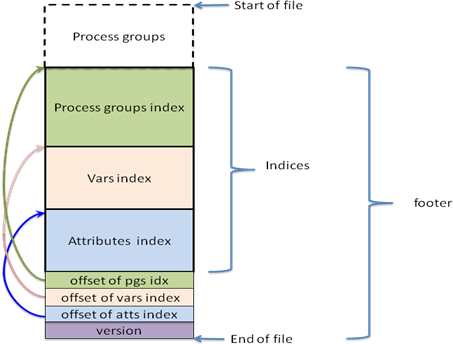
\includegraphics[width=217pt, height=163pt]{figures/bp-file-structure.png}
\caption{BP file structure}
\label{fig:bp-file-struct}
\end{center}
\end{figure}

\section{Footer}

One known limitation of the NetCDF format is that the file contents are stored 
in a header that is exactly big enough for the information provided at file creation. 
Any changes to the length of that data will require moving data. To avoid this 
cost, we choose to employ a foot index instead. We place our version identifier 
and the offset to the beginning of the index as the last few bytes of our file, 
making it simple to find the index information and to add new and different data 
to our files without affecting any data already written. 

\subsection{Version}

We reserve 4 bytes for the file version, in which the highest bit indicates endianness. 
Because ADIOS uses a fixed-size type for data, there is no need to store type size 
information in the footer. 

\subsection{Offsets of indices}

In BP format, we store three 8-byte file offsets right before the version word, 
which allows users or developers to quickly seek any of the index tables for process 
groups, variables, or attributes. 

\subsection{Indices}

\subsubsection{Characteristics}

Before we dive into the structures of the three index tables mentioned earlier, 
let's first take a look what characteristic means in terms of BP file format. To 
be able to make a summary inspection of the data to determine whether it contains 
the feature of greatest interest, we developed the idea of data characteristics. 
The idea of data characteristics is to collect some simple statistical and/or analytical 
data during the output operation or later for use in identifying the desired data 
sets. Simple statistics like array minimum and maximum values can be collected 
without extra overhead as part of the I/O operation. Other more complex analytical 
measures like standard deviations or specialized measures particular to the science 
being performance by require more processing. As part of our BP format, we store 
these values not only as part of data payload, but also in our index. 

\subsubsection{PG Index table}

As shown in Figure \ref{fig:group-index-table}, 
the process group (PG) index table encompasses the count 
and the total length of all the PGs as the first two entries. The rest of the tables 
contain a set of information for each PG, which contains the group name information, 
process ID, and time index. The Process ID specifies which process a group is written 
by. That process will be the rank value in the communicator if the MPI method is 
used. Most importantly, there is a file-offset entry for each PG, allowing a fast 
skip of the file in the unit of the process group.

\begin{figure}[htbp]
\begin{center}
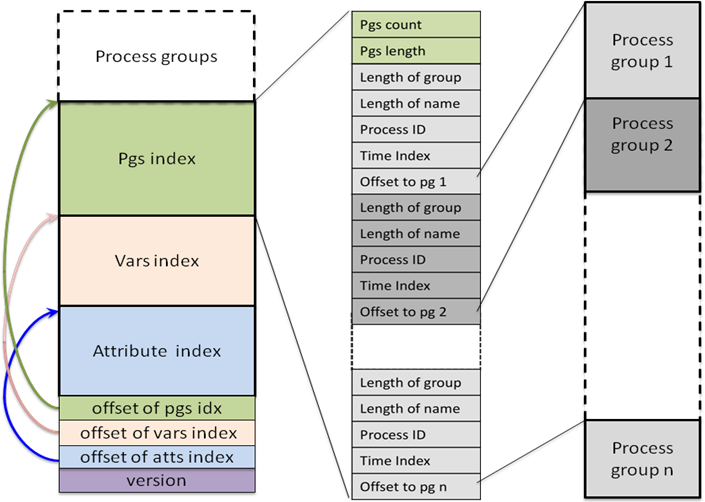
\includegraphics[width=338pt, height=238pt]{figures/group-index-table.png}
\caption{Group index table}
\label{fig:group-index-table}
\end{center}
\end{figure}

\subsubsection{Variables index table}

The variables index table is composed of the total count of variables in the BP 
file, the size of variables index table, and a list of variable records. Each record 
contains the size of the record and the basic metadata to describe the variable. 
As shown in Figure \ref{fig:variables-index-table}, 
the metadata include the name of the variable, the name 
of the group the variable is associated with, the data type of the variable, and 
a series of characteristic features. The structure of each characteristic entry 
contains an offset value, which is addressed to the certain occurrence of the variable 
in the BP file. For instance, if n processes write out the variable ``d'' per time 
step, and m iterations have been completed during the whole simulation, then the 
variable will be written (m\textit{ }\ensuremath{\times} n) times in the BP file 
that is produced. Accordingly, there will be the same number of elements in the 
list of characteristics. In this way, we can quickly retrieve the single dataset 
for all time steps or any other selection of time steps. This flexibility and efficiency 
also apply to a scenario in which a portion of records needs to be collected from 
a certain group of processes. 

\begin{figure}[htbp]
\begin{center}
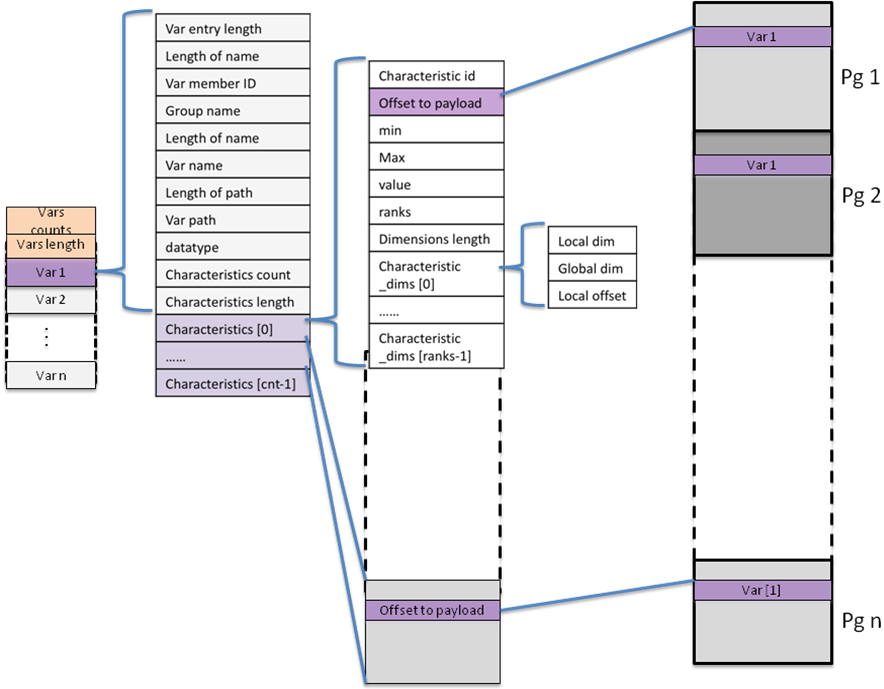
\includegraphics[width=420pt, height=327pt]{figures/variables-index-table.png}
\caption{Variables index table}
\label{fig:variables-index-table}
\end{center}
\end{figure}

\subsubsection{Attributes index table}

Since an attribute can be considered to be a special type of variable, its index 
table in BP format is organized in the same way as a variables index table and 
therefore supports the same types of features mentioned in the previous sections. 

\section{Process Groups}

One of the major concepts in BP format is what is called ``process group'' or PG. 
The BP file format encompasses a series of PG entries and the BP file footer. Each 
process group is the entire self-contained output from a single process and is 
written out independently into a contiguous disk space. In that way, we can enhance 
parallelism and reduce coordination among processes in the same communication group. 
The data diagram in Figure \ref{fig:process-group-struct} 
illustrates the detailed content in each PG. 

\begin{figure}[htbp]
\begin{center}
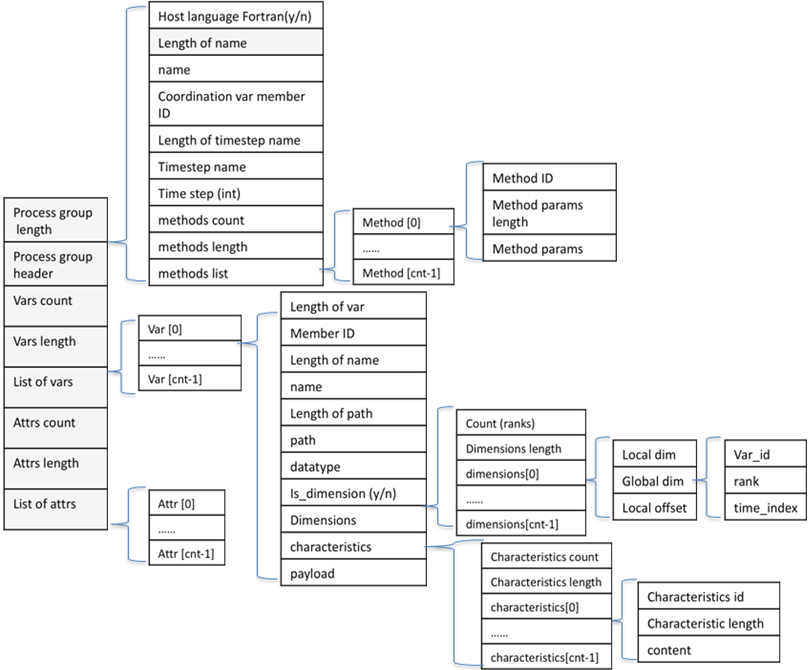
\includegraphics[width=389pt, height=321pt]{figures/process-group-structure.png}
\caption{Process group structure}
\label{fig:process-group-struct}
\end{center}
\end{figure}

\subsection{PG header}

\subsubsection{Unlimited dimension}

BP format allows users to define an unlimited dimension, which will be specified 
as the time-index in the XML file. Users can define variables having a dimension 
with undefined length, for which the variable can grow along that dimension. PG 
is a self-contained, independent data structure; the dataset in the local space 
per each time step is not reconstructed at the writing operations across the processes 
or at time steps. Theoretically, PGs can be appended to infinity; they can be added 
one after another no matter how many processes or time steps take place during 
the simulation.  Thus ADIOS is able to achieve high I/O performance.

\subsubsection{Transport methods}

One of the advantages of organizing output in terms of groups is to categorize 
all the variables based on their I/O patterns and logical relationships. It provides 
flexibility for each group to choose the optimized transport method according to 
the simulation environment and underlying hardware configuration or the transport 
methods used for a performance study without even changing the source code. In 
PG header structure, each entry in the method list has a method ID and method parameters, 
such as system-tuning parameters or underneath driver selection. 

\subsection{Vars list}

\subsubsection{Var header}

\emph{Dimensions structure.} 
Internal to bp is sufficient information to recreate any global structure and to 
place the local data into the structure. In the case of a global array, each process 
writes the size of the global array dimensions, specifies the local offsets into 
each, and then writes the local data, noting the size in each dimension. On conversion 
to another format, such as HDF5, this information is used to create hyperslabs 
for writing the data into the single, contiguous space. Otherwise, it is just read 
back in and used to note where the data came from. In this way, we can enhance 
parallelism and reduce coordination. All of our parallel writes occur independently 
unless the underlying transport specifically requires collective operations. Even 
in those cases, the collective calls are only for a full buffer write (assuming 
the transport was written appropriately) unless there is insufficient buffer space. 

As shown in Figure 19, the dimension structure contains a time index flag, which 
indicates whether this variable has an unlimited time dimension. Var\_id is used 
to retrieve the dimension value if the dimension is defined as variable in the 
XML file; otherwise, the rank value is taken as the array dimension.  

\subsubsection{Payload}

Basic statistical characteristics give users the advantage for quick data inspection 
and analysis. In Figure 19, redundant information about characteristics is stored 
along with variable payload so that if the characteristics part in the file footer 
gets corrupted, it can still be recovered quickly. Currently, only simple statistical 
traits are saved in the file, but the characteristics structure will be easily 
expanded or modified according to the requirements of scientific applications or 
the analysis tools. 

\subsection{Attributes list}

The layout of the attributes list (see Figure \ref{fig:attribute-entry-struct}) 
is very similar to that of the 
variables. However, instead of containing dimensional structures and physical data 
load, the attribute header has an is\_var flag, which indicates either that the 
value of the attribute is referenced from a variable by looking up the var\_id 
in the same group or that it is a static value defined in the XML file. 

\begin{figure}[htbp]
\begin{center}
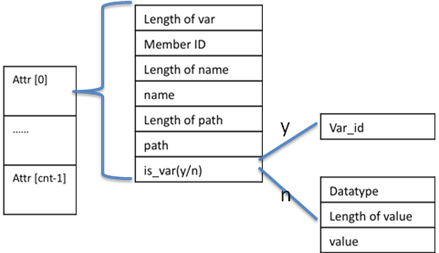
\includegraphics[width=210pt, height=120pt]{figures/attributes-entry-structure.png}
\caption{Attribute entry structure}
\label{fig:attribute-entry-struct}
\end{center}
\end{figure}



\vspace{36pt}
%\section*{{\Large \textbf{13 Developer Manual\label{HToc82067539}\label{HToc84890311}\label{HToc212016686}\label{HToc212016928}\label{HRef119999608}\label{HToc182553453}}}}
\section{Developer Manual}

\vspace{37pt}
\subsection*{{\large 13.1 }{\large \textbf{Create New Transport Methods}}}

\vspace{10pt}
One of ADIOS's important features is the componentization of transport methods. 
Users can switch among the typical methods that we support or even create their 
own methods, which can be easily plugged into our library. The following sections 
provide the procedures for adding the new transport method called ``abc'' into 
the ADIOS library. In this version of ADIOS, all the source files are located in 
/trunk/src/.\label{HToc84890312}\label{HToc212016687}\label{HToc212016929}\label{HToc182553454}

\vspace{10pt}
\subsubsection*{{\large \textbf{13.1.1 Add the new method macros in adios\_transport\_hooks.h 
}}}

\vspace{10pt}
The first file users need to examine is adios\_transport\_hooks.h, which basically 
defines all the transport methods and interface functions between detailed transport 
implementation and user APIs. In the file, we first find the line that defines 
the enumeration type Adios\_IO\_methods\_datatype add the declaration of method 
ID ADIOS\_METHOD\_ABC, and, because we add a new method, update total number of 
transport methods ADIOS\_METHOD\_COUNT from 9 to 10.

\vspace{10pt}
1. enum Adios\_IO\_methods datatype 

\vspace{10pt}
enum ADIOS\_IO\_METHOD \{

\vspace{10pt}
\parindent=79pt
ADIOS\_METHOD\_UNKNOWN   = -2

\vspace{10pt}
\parindent=75pt
,ADIOS\_METHOD\_NULL              = -1

\vspace{10pt}
,ADIOS\_METHOD\_MPI                 = 0

\vspace{23pt}
\parindent=226pt
,ADIOS\_METHOD\_PHDF5            = 8

\vspace{10pt}
\parindent=0pt
ADIOS\_METHOD\_ABC  = 9

\vspace{10pt}
\parindent=75pt
ADIOS\_METHOD\_COUNT           = 9   ADIOS\_METHOD\_COUNT  = 10

\vspace{10pt}
\};

\vspace{23pt}
\parindent=0pt
2. Next, we need to declare the transport APIs for method ``abc,'' including init/finalize, 
open/close, should\_buffer, and read/write. Similar to the other methods, we need 
to add 

\vspace{10pt}
\parindent=18pt
FORWARD\_DECLARE (abc)

\vspace{10pt}
\parindent=0pt
3. Then, we add the mapping of the string name ``abc'' of the new transport method 
to the method ID - ADIOS\_METHOD\_ABC, which has been already defined in enumeration 
type Adios\_IO\_methods\_datatype. As the last parameter, ``1'' here means the 
method requires communications, or ``0'' if not.

\vspace{10pt}
MATCH\_STRING\_TO\_METHOD (\texttt{"}abc\texttt{"}, ADIOS\_METHOD\_ABC, 1)     
        

\vspace{10pt}
4. Lastly, we add the mapping of the string name needed in the initialization functions 
to the method ID, which will be used by adios\_transport\_struct variables defined 
in adios\_internals.h.

\vspace{10pt}
ASSIGN\_FNS (abc, ADIOS\_METHOD\_ABC)\label{HToc84890313}\label{HToc212016688}\label{HToc212016930}\label{HToc182553455}

\vspace{10pt}
\subsubsection*{{\large \textbf{13.1.2 Create adios\_abc.c}}}

\vspace{10pt}
In this section, we demonstrate how to implement different transport APIs for method 
``abc.'' In adios\_abc.c, we need to implement at least 11 required routines: 

\vspace{10pt}
1. ``adios\_abc\_init'' allocates the method\_data field in adios\_method\_struct 
to the user-defined transport data structure, such as adios\_abc\_data\_struct, 
and initializes this data structure. Before the function returns, the initialization 
status can be set by statement ``adios\_abc\_initialized = 1.''

\vspace{10pt}
2. ``adios\_abc\_open'' opens a file if there is only one processor writing to 
the file. Otherwise, this function does nothing; instead, we use adios\_abc\_should\_buffer 
to coordinate the file open operations.   

\vspace{10pt}
3. ``adios\_abc\_should\_buffer,'' called by the ``common\_adios\_group\_size'' 
function in adios.c, needs to include coordination of open operations if multiple 
processes are writing to the same file. 

\vspace{10pt}
4. ``adios\_abc\_write'', in the case of no buffering or overflow, writes data 
directly to disk. Otherwise, it verifies whether the internally recorded memory 
pointer is consistent with the vector variable's address passed in the function 
parameter and frees that block of memory if it is not needed any more.  

\vspace{10pt}
5. ``adios\_abc\_read'' associates the internal data structure's address to the 
variable specified in the function parameter.

\vspace{10pt}
6. ``adios\_abc\_close'' simply closes the file if no buffering scheme is used. 
However, in general, this function performs most of the actual disk writing/reading 
the buffers to/from the file by one or more processors in the same communicator 
domain and then close the file. 

\vspace{10pt}
7. ``adios\_abc\_finalize'' resets the initialization status back to 0 if it has 
been set to 1 by adios\_abc\_init. 

\vspace{10pt}
If you are developing asynchronous methods, the following functions need to be 
implemented as well; otherwise you can leave them as empty implementation.

\vspace{10pt}
8. adios\_abc\_get\_write\_buffer,

\vspace{10pt}
9. ``adios\_abc\_end\_iteration`` is {\color{color01} a tick counter for the I/O 
routines to time how fast they are emptying the buffers.} 

\vspace{10pt}
10. ``adios\_abc\_start\_calculation'' {\color{color01} indicates that it is now 
an ideal time to do bulk data transfers because the code will not be performing 
I/O for a while.}

\vspace{10pt}
11. ``adios\_abc\_stop\_calculation`` indicates {\color{color01} that bulk data 
transfers should cease because the code is about to start communicating with other 
nodes.}

\vspace{10pt}
The following is One of the most important things that needs to be noted: 

\vspace{10pt}
fd-\texttt{>}shared\_buffer = adios\_flag\_no,

\vspace{10pt}
which means that the methods do not need a buffering scheme, such as PHDF5, and 
that data write out occurs immediately once adios\_write returns.

\vspace{10pt}
If fd-\texttt{>}shared\_buffer = adios\_flag\_yes, the users can employ the self-defined 
buffering scheme to improve I/O performance.\label{HToc84890314}\label{HToc212016689}\label{HToc212016931}\label{HToc182553456}

\vspace{10pt}
\subsubsection*{{\large \textbf{13.1.3 A walk-through example}}}

\vspace{10pt}
Now let's look at an example of adding an unbuffered POSIX method to ADIOS.  According 
to the steps described above, we first open the header file --``adios\_transport\_hooks.h,'' 
and add the following statements:

\vspace{10pt}
\ensuremath{\Sigma} \textbf{enum ADIOS\_IO\_METHOD} \{

\vspace{10pt}
\parindent=79pt
ADIOS\_METHOD\_UNKNOWN     = -2

\vspace{10pt}
\parindent=75pt
,ADIOS\_METHOD\_NULL                 = -1

\vspace{10pt}
,ADIOS\_METHOD\_MPI                    = 0...

\vspace{23pt}
\parindent=226pt
,ADIOS\_METHOD\_PROVENANCE  = 8

\vspace{10pt}
\parindent=0pt
// method ID for binary transport method

\vspace{10pt}
\parindent=75pt
\textbf{,ADIOS\_METHOD\_POSIX\_ASCII\_NB  = 9 }

\vspace{10pt}
// total method number

\vspace{10pt}
\textbf{,ADIOS\_METHOD\_COUNT  = 10 }

\vspace{10pt}
\};

\vspace{10pt}
\parindent=0pt
\ensuremath{\Sigma} \textbf{FORWARD\_DECLARE (posix\_ascii\_nb);}

\vspace{23pt}
\ensuremath{\Sigma} \textbf{MATCH\_STRING\_TO\_METHOD (\texttt{"}posix\_ascii\_nb\texttt{"}}

\vspace{10pt}
\textbf{, ADIOS\_METHOD\_ POSIX\_ASCII\_NB, 0)}

\vspace{10pt}
\ensuremath{\Sigma} \textbf{ASSIGN\_FNS (binary, ADIOS\_METHOD\_ POSIX\_ASCII\_NB)}

\vspace{10pt}
Next, we must create adios\_posix\_ascii\_nb,c, which defines all the required 
routines listed in Sect. 12.1.2 The blue highlights below mark out the data structures 
and required functions that developers need to implement in the source code. 

\vspace{23pt}
static int adios\_posix\_ascii\_nb\_initialized{\color{color02}  }= 0;

\vspace{10pt}
struct {\color{color02} adios\_POSIX\_ASCII\_UNBUFFERED\_data\_struct }

\vspace{10pt}
\{

\vspace{10pt}
\parindent=14pt
FILE *f;

\vspace{10pt}
uint64\_t file\_size;

\vspace{10pt}
\parindent=0pt
\};

\vspace{23pt}
void {\color{color02} adios\_posix\_ascii\_nb \_init} {\color{color02} (const char 
*parameters}

\vspace{10pt}
\parindent=183pt
{\color{color02} , struct adios\_method\_struct * method) }

\vspace{10pt}
\parindent=0pt
\{

\vspace{10pt}
\parindent=14pt
struct adios\_POSIX\_ASCII\_UNBUFFERED\_data\_struct * md;

\vspace{10pt}
if (!adios\_posix\_ascii\_nb\_initialized)

\vspace{10pt}
\parindent=28pt
\{

\vspace{10pt}
adios\_posix\_ascii\_nb\_initialized = 1;

\vspace{10pt}
\parindent=43pt
\}

\vspace{10pt}
\parindent=14pt
method-\texttt{>}method\_data = malloc (

\vspace{10pt}
\parindent=147pt
sizeof(struct adios\_POSIX\_ASCII\_UNBUFFERED\_data\_struct)

\vspace{10pt}
\parindent=237pt
);

\vspace{10pt}
\parindent=14pt
md = (struct adios\_POSIX\_ASCII\_UNBUFFERED\_data\_struct *) 

\vspace{10pt}
\parindent=165pt
method-\texttt{>}method\_data;      

\vspace{10pt}
\parindent=14pt
md-\texttt{>}f = 0;

\vspace{10pt}
md-\texttt{>}file\_size = 0;

\vspace{10pt}
\}

\vspace{23pt}
int {\color{color02} adios\_posix\_ascii\_nb \_open (struct adios\_file\_struct 
* fd}

\vspace{10pt}
\parindent=133pt
{\color{color02} , struct adios\_method\_struct * method)}

\vspace{10pt}
\parindent=0pt
\{

\vspace{10pt}
\parindent=14pt
char * name;

\vspace{10pt}
struct adios\_POSIX\_ASCII\_UNBUFFERED\_data\_struct * p;

\vspace{10pt}
\parindent=28pt
struct stat s;

\vspace{10pt}
\parindent=14pt
p = (struct adios\_POSIX\_ASCII\_UNBUFFERED\_data\_struct *)

\vspace{10pt}
\parindent=208pt
method-\texttt{>}method\_data;

\vspace{10pt}
\parindent=14pt
name = malloc (strlen (method-\texttt{>}base\_path) + strlen (fd-\texttt{>}name) 
+ 1);

\vspace{10pt}
sprintf (name, \texttt{"}\%s\%s\texttt{"}, method-\texttt{>}base\_path, fd-\texttt{>}name);

\vspace{10pt}
\parindent=28pt
if (stat (name, \&s) == 0)

\vspace{10pt}
p-\texttt{>}file\_size = s.st\_size;

\vspace{10pt}
\parindent=43pt
switch (fd-\texttt{>}mode)

\vspace{10pt}
\parindent=14pt
\{

\vspace{10pt}
\parindent=28pt
case adios\_mode\_read:

\vspace{10pt}
\{

\vspace{10pt}
\parindent=72pt
p-\texttt{>}f = fopen (name, \texttt{"}r\texttt{"});

\vspace{10pt}
\parindent=43pt
if (p-\texttt{>}f \texttt{<}= 0)

\vspace{10pt}
\{

\vspace{10pt}
\parindent=100pt
fprintf (stderr, \texttt{"}ADIOS POSIX ASCII UNBUFFERED: \texttt{"}

\vspace{10pt}
\parindent=118pt
\texttt{"}file not found: \%s\textbackslash{}n\texttt{"}, fd-\texttt{>}name);

\vspace{10pt}
\parindent=57pt
free (name);

\vspace{10pt}
return 0;

\vspace{10pt}
\parindent=100pt
\}

\vspace{10pt}
\parindent=43pt
break;

\vspace{10pt}
\parindent=28pt
\}

\vspace{10pt}
case adios\_mode\_write:

\vspace{10pt}
\parindent=57pt
\{

\vspace{10pt}
\parindent=43pt
p-\texttt{>}f = fopen (name, \texttt{"}w\texttt{"});

\vspace{10pt}
if (p-\texttt{>}f \texttt{<}= 0)

\vspace{10pt}
\parindent=86pt
\{

\vspace{10pt}
\parindent=57pt
fprintf (stderr, \texttt{"}adios\_posix\_ascii\_nb\_open \texttt{"}

\vspace{10pt}
\parindent=111pt
\texttt{"}failed for base\_path \%s, name \%s\textbackslash{}n\texttt{"}

\vspace{10pt}
\parindent=0pt
,method-\texttt{>}base\_path, fd-\texttt{>}name

\vspace{10pt}
);

\vspace{10pt}
\parindent=57pt
free (name);

\vspace{10pt}
return 0;

\vspace{10pt}
\parindent=100pt
\}

\vspace{10pt}
\parindent=43pt
break;

\vspace{10pt}
\parindent=28pt
\} 

\vspace{10pt}
case adios\_mode\_append:

\vspace{10pt}
\parindent=57pt
\{

\vspace{10pt}
\parindent=43pt
int old\_file = 1;

\vspace{10pt}
p-\texttt{>}f = fopen (name, \texttt{"}a\texttt{"});

\vspace{10pt}
\parindent=86pt
if (p-\texttt{>}f \texttt{<}= 0)

\vspace{10pt}
\parindent=43pt
\{

\vspace{10pt}
\parindent=57pt
fprintf (stderr, \texttt{"}adios\_posix\_ascii\_nb\_open\texttt{"}

\vspace{10pt}
\parindent=118pt
\texttt{"} failed for base\_path \%s, name \%s\textbackslash{}n\texttt{"}

\vspace{10pt}
\parindent=86pt
,method-\texttt{>}base\_path, fd-\texttt{>}name

\vspace{10pt}
);

\vspace{10pt}
\parindent=144pt
free (name);

\vspace{10pt}
\parindent=57pt
return 0;

\vspace{10pt}
\parindent=43pt
\}

\vspace{10pt}
break;

\vspace{10pt}
\parindent=72pt
\}

\vspace{10pt}
\parindent=28pt
default:

\vspace{10pt}
\{

\vspace{10pt}
\parindent=72pt
fprintf (stderr, \texttt{"}Unknown file mode: \%d\textbackslash{}n\texttt{"}, fd-\texttt{>}mode);

\vspace{10pt}
\parindent=43pt
free (name);

\vspace{10pt}
return 0;

\vspace{10pt}
\parindent=72pt
\}

\vspace{10pt}
\parindent=14pt
\}

\vspace{10pt}
free (name);

\vspace{10pt}
\parindent=28pt
return 0;

\vspace{10pt}
\parindent=0pt
\}

\vspace{23pt}
enum ADIOS\_FLAG {\color{color02} \textbf{adios\_posix\_ascii\_nb\_should\_buffer}}{\color{color02}  
}

\vspace{10pt}
\parindent=205pt
{\color{color02} (struct adios\_file\_struct * fd}

\vspace{10pt}
{\color{color02} ,struct adios\_method\_struct * method}

\vspace{10pt}
\parindent=410pt
{\color{color02} ,void * comm) }

\vspace{10pt}
\parindent=0pt
\{

\vspace{10pt}
\parindent=14pt
//in this case, we don't use shared\_buffer

\vspace{10pt}
return adios\_flag\_no;

\vspace{10pt}
\parindent=0pt
\}

\vspace{23pt}
void {\color{color02} \textbf{adios\_posix\_ascii\_nb\_write}} (struct adios\_file\_struct 
* fd

\vspace{10pt}
\parindent=158pt
,struct adios\_var\_struct * v 

\vspace{10pt}
,void * data

\vspace{10pt}
\parindent=316pt
,struct adios\_method\_struct * method ) 

\vspace{10pt}
\parindent=0pt
\{

\vspace{10pt}
\parindent=14pt
struct adios\_POSIX\_ASCII\_UNBUFFERED\_data\_struct * p;

\vspace{10pt}
p = (struct adios\_POSIX\_ASCII\_UNBUFFERED\_data\_struct *)

\vspace{10pt}
\parindent=154pt
method-\texttt{>}method\_data;

\vspace{10pt}
\parindent=14pt
if (!v-\texttt{>}dimensions) \{

\vspace{10pt}
\parindent=28pt
switch (v-\texttt{>}type)

\vspace{10pt}
\{

\vspace{10pt}
\parindent=72pt
case adios\_byte:

\vspace{10pt}
\parindent=43pt
case adios\_unsigned\_byte:

\vspace{10pt}
\parindent=57pt
fprintf (p-\texttt{>}f,\texttt{"}\%c\textbackslash{}n\texttt{"}, *((char *)data)); 

\vspace{10pt}
break;

\vspace{10pt}
\parindent=100pt
case adios\_short:

\vspace{10pt}
\parindent=43pt
case adios\_integer:

\vspace{10pt}
case adios\_unsigned\_short:

\vspace{10pt}
\parindent=86pt
case adios\_unsigned\_integer:

\vspace{10pt}
\parindent=57pt
fprintf (p-\texttt{>}f,\texttt{"}\%d\textbackslash{}n\texttt{"}, *((int *)data)); 

\vspace{10pt}
break;

\vspace{10pt}
\parindent=100pt
case adios\_real:

\vspace{10pt}
\parindent=43pt
case adios\_double:

\vspace{10pt}
case adios\_long\_double:

\vspace{10pt}
\parindent=100pt
fprintf (p-\texttt{>}f,\texttt{"}\%f\textbackslash{}n\texttt{"}, *((double *)data)); 

\vspace{10pt}
\parindent=57pt
break;

\vspace{10pt}
\parindent=43pt
case adios\_string:

\vspace{10pt}
\parindent=57pt
fprintf (p-\texttt{>}f,\texttt{"}\%s\textbackslash{}n\texttt{"}, (char *)data); 

\vspace{10pt}
break;

\vspace{10pt}
\parindent=100pt
case adios\_complex:

\vspace{10pt}
\parindent=57pt
fprintf (p-\texttt{>}f,\texttt{"}\%f+\%fi\textbackslash{}n\texttt{"}, *((float 
*)data),*((float *)(data+4))); 

\vspace{10pt}
break;

\vspace{10pt}
\parindent=100pt
case adios\_double\_complex:

\vspace{10pt}
\parindent=57pt
fprintf (p-\texttt{>}f,\texttt{"}\%f+\%fi\textbackslash{}n\texttt{"}, *((double 
*)data),*((double *)(data+8))); 

\vspace{10pt}
break;

\vspace{10pt}
\parindent=3pt
default:

\vspace{10pt}
\parindent=57pt
break;

\vspace{10pt}
\parindent=18pt
\}

\vspace{10pt}
\parindent=14pt
\} 

\vspace{10pt}
else

\vspace{10pt}
\parindent=28pt
\{

\vspace{10pt}
uint64\_t j;

\vspace{10pt}
\parindent=57pt
int element\_size = adios\_get\_type\_size (v-\texttt{>}type, v-\texttt{>}data);

\vspace{10pt}
\parindent=28pt
printf(\texttt{"}element\_size: \%d\textbackslash{}n\texttt{"},element\_size);

\vspace{10pt}
uint64\_t var\_size = adios\_get\_var\_size (v, fd-\texttt{>}group, v-\texttt{>}data)/element\_size;

\vspace{10pt}
\parindent=57pt
switch (v-\texttt{>}type)

\vspace{10pt}
\parindent=28pt
\{

\vspace{10pt}
\parindent=43pt
case adios\_byte:

\vspace{10pt}
case adios\_unsigned\_byte:

\vspace{10pt}
\parindent=100pt
for (j = 0;j \texttt{<} var\_size; j++)

\vspace{10pt}
\parindent=72pt
fprintf (p-\texttt{>}f,\texttt{"}\%c \texttt{"}, *((char *)(data+j)));

\vspace{10pt}
\parindent=57pt
printf(\texttt{"}\textbackslash{}n\texttt{"});

\vspace{10pt}
break;

\vspace{10pt}
\parindent=100pt
case adios\_short:

\vspace{10pt}
\parindent=43pt
case adios\_integer:

\vspace{10pt}
case adios\_unsigned\_short:

\vspace{10pt}
\parindent=86pt
case adios\_unsigned\_integer:

\vspace{10pt}
\parindent=57pt
for (j = 0;j \texttt{<} var\_size; j++)

\vspace{10pt}
\parindent=72pt
fprintf (p-\texttt{>}f,\texttt{"}\%d \texttt{"}, *((int *)(data+element\_size*j)));

\vspace{10pt}
\parindent=57pt
printf(\texttt{"}\textbackslash{}n\texttt{"});

\vspace{10pt}
break;

\vspace{10pt}
\parindent=100pt
case adios\_real:

\vspace{10pt}
\parindent=43pt
case adios\_double:

\vspace{10pt}
case adios\_long\_double:

\vspace{10pt}
\parindent=100pt
for (j = 0;j \texttt{<} var\_size; j++)

\vspace{10pt}
\parindent=72pt
fprintf (p-\texttt{>}f,\texttt{"}\%f \texttt{"}, * ( (double *)(data+element\_size*j)) 
);

\vspace{10pt}
\parindent=57pt
printf(\texttt{"}\textbackslash{}n\texttt{"});

\vspace{10pt}
break;

\vspace{10pt}
\parindent=100pt
case adios\_string:

\vspace{10pt}
\parindent=57pt
for (j = 0;j \texttt{<} var\_size; j++)

\vspace{10pt}
\parindent=72pt
fprintf (p-\texttt{>}f,\texttt{"}\%s \texttt{"}, (char *)data);

\vspace{10pt}
\parindent=57pt
printf(\texttt{"}\textbackslash{}n\texttt{"});

\vspace{10pt}
break;

\vspace{10pt}
\parindent=100pt
case adios\_complex:

\vspace{10pt}
\parindent=57pt
for (j = 0;j \texttt{<} var\_size; j++)

\vspace{10pt}
\parindent=72pt
fprintf (p-\texttt{>}f, \texttt{"}\%f+\%fi \texttt{"}, *((float *)(data+element\_size*j))

\vspace{10pt}
\parindent=100pt
,*((float *)(data+4+element\_size*j))

\vspace{10pt}
);

\vspace{10pt}
\parindent=158pt
printf(\texttt{"}\textbackslash{}n\texttt{"});

\vspace{10pt}
\parindent=57pt
break;

\vspace{10pt}
\parindent=43pt
case adios\_double\_complex:

\vspace{10pt}
\parindent=57pt
for (j = 0;j \texttt{<} var\_size; j++)

\vspace{10pt}
\parindent=72pt
fprintf (p-\texttt{>}f,\texttt{"}\%f+\%fi \texttt{"}, *((double *)(data+element\_size*j))

\vspace{10pt}
\parindent=100pt
,*((double *)(data+element\_size*j+8)));

\vspace{10pt}
\parindent=57pt
printf(\texttt{"}\textbackslash{}n\texttt{"});

\vspace{10pt}
break;

\vspace{10pt}
\parindent=100pt
default:

\vspace{10pt}
\parindent=57pt
break;

\vspace{10pt}
\parindent=28pt
\} 

\vspace{10pt}
\parindent=14pt
\}

\vspace{10pt}
\parindent=0pt
\}

\vspace{23pt}
\parindent=100pt
void {\color{color02} \textbf{adios\_posix\_ascii\_nb\_get\_write\_buffer }}

\vspace{10pt}
\parindent=190pt
{\color{color02} (struct adios\_file\_struct * fd}

\vspace{10pt}
\parindent=194pt
{\color{color02} ,struct adios\_var\_struct * v}

\vspace{10pt}
{\color{color02} ,uint64\_t * size}

\vspace{10pt}
\parindent=388pt
{\color{color02} ,void ** buffer}

\vspace{10pt}
\parindent=194pt
{\color{color02} ,struct adios\_method\_struct * method) }

\vspace{10pt}
\parindent=0pt
\{

\vspace{10pt}
\parindent=14pt
*buffer = 0;

\vspace{10pt}
\parindent=0pt
\}

\vspace{23pt}
void {\color{color02} \textbf{adios\_posix\_ascii\_nb\_read}}\textbf{ }{\color{color02} (struct 
adios\_file\_struct * fd}

\vspace{10pt}
\parindent=115pt
{\color{color02} ,struct adios\_var\_struct * v, void * buffer}

\vspace{10pt}
\parindent=118pt
{\color{color02} ,uint64\_t buffer\_size}

\vspace{10pt}
{\color{color02} ,struct adios\_method\_struct * method )}

\vspace{10pt}
\parindent=0pt
\{

\vspace{10pt}
\parindent=14pt
v-\texttt{>}data = buffer;

\vspace{10pt}
v-\texttt{>}data\_size = buffer\_size; 

\vspace{10pt}
\parindent=0pt
\}

\vspace{23pt}
\textbf{int}{\color{color02} \textbf{ adios\_posix\_ascii\_nb\_close}} {\color{color02} (struct 
adios\_file\_struct * fd}

\vspace{10pt}
\parindent=194pt
{\color{color02} , struct adios\_method\_struct * method)}

\vspace{10pt}
\parindent=0pt
\{

\vspace{10pt}
struct adios\_POSIX\_ASCII\_UNBUFFERED\_data\_struct * p;

\vspace{10pt}
\parindent=14pt
p = (struct adios\_POSIX\_ASCII\_UNBUFFERED\_data\_struct *)

\vspace{10pt}
\parindent=208pt
method-\texttt{>}method\_data;

\vspace{10pt}
\parindent=14pt
if (p-\texttt{>}f \texttt{<}= 0)

\vspace{10pt}
\{

\vspace{10pt}
\parindent=43pt
fclose (p-\texttt{>}f);

\vspace{10pt}
\parindent=14pt
\}

\vspace{10pt}
p-\texttt{>}f = 0;

\vspace{10pt}
\parindent=28pt
p-\texttt{>}file\_size = 0; 

\vspace{10pt}
\parindent=0pt
\}

\vspace{23pt}
void {\color{color02} \textbf{adios\_posix\_ascii\_nb\_finalize}}\textbf{ }{\color{color02} (int 
mype, struct adios\_method\_struct * method)} 

\vspace{10pt}
\{

\vspace{10pt}
\parindent=14pt
if (adios\_posix\_ascii\_nb\_initialized)

\vspace{10pt}
\parindent=28pt
adios\_posix\_ascii\_nb\_initialized = 0; 

\vspace{10pt}
\parindent=0pt
\}

\vspace{36pt}
The binary transport method blocks methods for simplicity. Therefore,  no special 
implementation for the three functions below is necessary and their function bodies 
can be left empty:

\vspace{23pt}
{\color{color02} \textbf{adios\_posix\_ascii\_nb\_end\_iteration}}{\color{color02}  
(struct adios\_method\_struct * method) }\{\}

\vspace{10pt}
{\color{color02} \textbf{adios\_posix\_ascii\_nb\_start\_calculation}}{\color{color02}  
(struct adios\_method\_struct * method) }\{\}

\vspace{10pt}
{\color{color02} \textbf{adios posix\_ascii\_nb stop\_calculation}}{\color{color02}  
(struct adios\_method\_struct * method)} \{\}

\vspace{23pt}
Above, we have implemented the POSIX\_ASCII\_NB transport method. When users specify 
POSIX\_ASCII\_NB method in xml file, the users' applications will generate ASCII 
files by using common ADIOS APIs. However, in order to achieve better I/O performance, 
a buffering scheme needs to be included into this example.\label{HToc82067540}\label{HToc84890315}\label{HToc212016690}\label{HToc212016932}\label{HToc182553457}

\vspace{10pt}
\subsection*{{\large 13.2 }{\large \textbf{Profiling the Application and ADIOS}}}

\vspace{10pt}
There are two ways to get profiling information of ADIOS I/O operations. One way 
is for the user to explicitly insert a set of profiling API calls around ADIOS 
API calls in the source code. The other way is to link the user code with a renamed 
ADIOS library and an ADIOS API wrapper library. \label{HToc84890316}\label{HToc212016691}\label{HToc212016933}\label{HToc182553458}

\vspace{10pt}
\subsubsection*{{\large \textbf{13.2.1 Use profiling API in source code}}}

\vspace{10pt}
The profiling library called libadios\_timing.a implements a set of profiling API 
calls. The user can use these API calls to wrap the ADIOS API calls in the source 
code to get profiling information. 

\vspace{10pt}
The adios-timing.h header file contains the declarations of those profiling functions. 

\vspace{10pt}
\begin{longtable}{|p{4.448in}|p{0.052in}|}
\hline
% ROW 1
\begin{minipage}[t]{4.448in}\raggedright /*\linebreak
* initialize profiling \linebreak
*\linebreak
* Fortran interface\linebreak
*/\linebreak
int init\_prof\_all\_(char *prof\_file\_name, int prof\_file\_name\_size);\linebreak
/*\linebreak
* record open start time for specified group\linebreak
*\linebreak
* Fortran interface\linebreak
*/\linebreak
void open\_start\_for\_group\_(int64\_t *gp\_prof\_handle, char *group\_name, int 
*cycle, int *gp\_name\_size);\linebreak
/*\linebreak
* record open end time for specified group\linebreak
*\linebreak
* Fortran interface\linebreak
*/\linebreak
void open\_end\_for\_group\_(int64\_t *gp\_prof\_handle, int *cycle);\linebreak
/*\linebreak
* record write start time for specified group\linebreak
*\linebreak
* Fortran interface\linebreak
*/\linebreak
void write\_start\_for\_group\_(int64\_t *gp\_prof\_handle, int *cycle);\linebreak
/*\linebreak
* record write end time for specified group\linebreak
*\linebreak
* Fortran interface\linebreak
*/\linebreak
void write\_end\_for\_group\_(int64\_t *gp\_prof\_handle, int *cycle);\linebreak
/*\linebreak
* record close start time for specified group\linebreak
*\linebreak
* Fortran interface\linebreak
*/\linebreak
void close\_start\_for\_group\_(int64\_t *gp\_prof\_handle, int *cycle);\linebreak
/*\linebreak
* record close end time for specified group\linebreak
*\linebreak
* Fortran interface\linebreak
*/\linebreak
void close\_end\_for\_group\_(int64\_t *gp\_prof\_handle, int *cycle);\linebreak
/*\linebreak
* Report timing info for all groups\linebreak
*\linebreak
* Fortran interface  \linebreak
*/\linebreak
int finalize\_prof\_all\_();\linebreak
/*\linebreak
* record start time of a simulation cycle\linebreak
*\linebreak
* Fortran interface \linebreak
*/\linebreak
void cycle\_start\_(int *cycle);\linebreak
/*\linebreak
* record end time of a simulation cycle\linebreak
*\linebreak
* Fortran interface \linebreak
*/\linebreak
void cycle\_end\_(int *cycle);\end{minipage}\\
\hline
\end{longtable}

\vspace{142pt}
An example of using these functions is given below....

\vspace{23pt}
! initialization ADIOS

\vspace{10pt}
CALL adios\_init (\texttt{"}config.xml\texttt{"}//char(0))

\vspace{10pt}
! initialize profiling library; the parameter specifies the file where profiling 
information is written

\vspace{10pt}
CALL init\_prof\_all(\texttt{"}log\texttt{"}//char(0))...

\vspace{23pt}
CALL MPI\_Barrier(toroidal\_comm, error )

\vspace{23pt}
! record start time of open

\vspace{10pt}
! group\_prof\_handle is an OUT parameter holding the handle for the group `output3d.0'

\vspace{10pt}
! istep is iteration no.

\vspace{10pt}
CALL open\_start\_for\_group(group\_prof\_handle, \texttt{"}output3d.0\texttt{"}//char(0),istep)

\vspace{23pt}
CALL adios\_open(adios\_handle, \texttt{"}output3d.0\texttt{"}//char(0), ``w''//char(0))

\vspace{23pt}
! record end time of open

\vspace{10pt}
CALL open\_end\_for\_group(group\_prof\_handle,istep)

\vspace{23pt}
! record start time of write

\vspace{10pt}
CALL write\_start\_for\_group(group\_prof\_handle,istep)

\vspace{23pt}
\#include \texttt{"}gwrite\_output3d.0.fh\texttt{"}

\vspace{23pt}
! record end time of write

\vspace{10pt}
CALL write\_end\_for\_group(group\_prof\_handle,istep)

\vspace{23pt}
! record start time of close

\vspace{10pt}
CALL cose\_start\_for\_group(group\_prof\_handle,istep)

\vspace{23pt}
CALL adios\_close(adios\_handle,adios\_err)

\vspace{23pt}
! record end time of close

\vspace{10pt}
CALL close\_end\_for\_group(group\_prof\_handle,istep)...

\vspace{36pt}
CALL adios\_finalize (myid)

\vspace{23pt}
! finalize; profiling information are gathered and min/max/mean/var are calculated 
for each IO dump

\vspace{10pt}
CALL finalize\_prof()

\vspace{23pt}
CALL MPI\_FINALIZE(error)

%\vspace{10pt}
%\begin{longtable}{|p{4.500in}|}
%\hline
% ROW 1
%\begin{minipage}[t]{4.500in}\raggedright 
%\hline
%\end{longtable}

\vspace{23pt}
When the code is run, profiling information will be saved to the file ''./log'' 
(specified in init\_prof\_all ()). Below is an example.

\vspace{10pt}
{\small Fri Aug 22 15:42:04 EDT 2008}

\vspace{10pt}
{\small I/O Timing results}

\vspace{10pt}
{\small Operations    :          min                     max                   
  mean                    var}

\vspace{10pt}
{\small cycle no         3}

\vspace{10pt}
{\small io count         0}

\vspace{10pt}
{\small \# Open        :          0.107671                0.108245             
   0.108032                0.000124}

\vspace{10pt}
{\small \# Open start  :          1219434228.866144       1219434230.775268    
   1219434229.748614       0.588501}

\vspace{10pt}
{\small \# Open end    :          1219434228.974225       1219434230.883335    
   1219434229.856646       0.588486}

\vspace{10pt}
{\small \# Write       :          0.000170                0.000190             
   0.000179                0.000005}

\vspace{10pt}
{\small \# Write start :          1219434228.974226       1219434230.883336    
   1219434229.856647       0.588486}

\vspace{10pt}
{\small \# Write end   :          1219434228.974405       1219434230.883514    
   1219434229.856826       0.588484}

\vspace{10pt}
{\small \# Close       :          0.001608                0.001743             
   0.001656                0.000036}

\vspace{10pt}
{\small \# Close start :          1219434228.974405       1219434230.883514    
   1219434229.856826       0.588484}

\vspace{10pt}
{\small \# Close end   :          1219434228.976040       1219434230.885211    
   1219434229.858482       0.588489}

\vspace{10pt}
{\small \# Total       :          0.109484                0.110049             
   0.109868                0.000137}

\vspace{10pt}
{\small cycle no         6}

\vspace{10pt}
{\small io count         1}

\vspace{10pt}
{\small \# Open        :          0.000007                0.000011             
   0.000009                0.000001}

\vspace{10pt}
{\small \# Open start  :          1219434240.098444       1219434242.007951    
   1219434240.981075       0.588556}

\vspace{10pt}
{\small \# Open end    :          1219434240.098452       1219434242.007962    
   1219434240.981083       0.588556}

\vspace{10pt}
{\small \# Write       :          0.000175                0.000196             
   0.000180                0.000004}

\vspace{10pt}
{\small \# Write start :          1219434240.098452       1219434242.007962    
   1219434240.981083       0.588557}

\vspace{10pt}
{\small \# Write end   :          1219434240.098631       1219434242.008158    
   1219434240.981264       0.588558}

\vspace{10pt}
{\small \# Close       :          0.000947                0.003603             
   0.001234                0.000466}

\vspace{10pt}
{\small \# Close start :          1219434240.098631       1219434242.008158    
   1219434240.981264       0.588558}

\vspace{10pt}
{\small \# Close end   :          1219434240.099665       1219434242.009620    
   1219434240.982498       0.588447}

\vspace{10pt}
{\small \# Total       :          0.001132                0.003789             
   0.001423                0.000466}

%\vspace{10pt}
%\begin{longtable}{|p{4.500in}|}
%\hline
% ROW 1
%\begin{minipage}[t]{4.500in}\raggedright \\
%\hline
%\end{longtable}

\vspace{23pt}
The script ``post\_script.sh'' extracts ``open time'', ``write time'', ``close 
time'', and ``total time'' from the raw profiling results and saves them in separate 
files: open, write, close, and total, respectively.\label{HToc212016692}\label{HToc212016815}\label{HToc212016934}\label{HToc212018088}

\vspace{10pt}
To compile the code, one should link the code with the -\textit{ladios\_timing 
-ladios} option. \label{HToc84890317}\label{HToc212016693}\label{HToc212016935}\label{HToc182553459}

\vspace{10pt}
\subsubsection*{{\large \textbf{13.2.2 Use wrapper library}}}

\vspace{10pt}
Another way to do profiling is to link the source code with a renamed ADIOS library 
and a wrapper library. 

\vspace{10pt}
The renamed ADIOS library implements ``real'' ADIOS routines, but all ADIOS public 
functions are renamed with a prefix ``P''. For example, adios\_open() is renamed 
as Padios\_open(). The routine for parsing config.xml file is also changed to parse 
extra flags in config.xml file to turn profiling on or off.

\vspace{10pt}
The wrapper library implements all adios pubic functions (e.g., adios\_open, adios\_write, 
adios\_close) within each function. It calls the ``real'' function (Padios\_xxx()) 
and measure the start and end time of the function call. 

\vspace{10pt}
There is an example wrapper library called libadios\_profiling.a. Developers can 
implement their own wrapper library to customize the profiling.

\vspace{10pt}
To use the wrapper library, the user code should be linked with -\textit{ladios\_profiling 
-ladios}. the wrapper library should precede the ``real'' ADIOS library. There 
is no need to put additional profiling API calls in the source code. The user can 
turn profiling on or off for each ADIOS group by setting a flag in the config.xml 
file.

\vspace{10pt}
\texttt{<}adios-group name=\texttt{"}restart.model\texttt{"} profiling=``yes\textbar{}no\texttt{"}\texttt{>}

\vspace{10pt}
\parindent=14pt
...

\vspace{10pt}
\parindent=0pt
\texttt{<}/adios-group\texttt{>}

%\vspace{10pt}
%\begin{longtable}{|p{4.500in}|}
%\hline
% ROW 1
%\begin{minipage}[t]{4.500in}\raggedright \\
%\hline
%\end{longtable}
\label{HToc84890323}\label{HToc212016699}\label{HToc212016942}\label{HToc182553460}


\chapter{Appendix}
\label{section-appendix}

\section{Datatypes used in the ADIOS XML file}

\section*{\begin{longtable}{llllll}
\hline
% ROW 1
\multicolumn{1}{|p{0.287in}|}{\begin{minipage}[t]{0.287in}\centering
{\small \textbf{size}}\end{minipage}} & \multicolumn{1}{p{2.534in}|}{\begin{minipage}[t]{2.534in}\centering
{\small \textbf{Signed type}}\end{minipage}} & \multicolumn{1}{p{1.526in}|}{\begin{minipage}[t]{1.526in}\raggedright
{\small \textbf{Unsigned type}}\end{minipage}}\\
\hline
% ROW 2
\multicolumn{1}{p{0.051in}|}{\begin{minipage}[t]{0.051in}\centering
{\small 1}\end{minipage}} & \multicolumn{1}{p{0.051in}|}{\begin{minipage}[t]{0.051in}\centering
{\small byte, interger*1}\end{minipage}} & \multicolumn{1}{p{0.051in}|}{\begin{minipage}[t]{0.051in}\centering
{\small unsigned byte, unsigned integer*1}\end{minipage}}\\
\hline
% ROW 3
\multicolumn{1}{|p{0.287in}|}{\begin{minipage}[t]{0.287in}\centering
{\small 2}\end{minipage}} & \multicolumn{1}{p{2.534in}|}{\begin{minipage}[t]{2.534in}\centering
{\small short, integer*2}\end{minipage}} & \multicolumn{1}{p{1.526in}|}{\begin{minipage}[t]{1.526in}\raggedright
{\small unsigned short, unsigned integer*2}\end{minipage}}\\
\hline
% ROW 4
\multicolumn{1}{p{0.051in}|}{\begin{minipage}[t]{0.051in}\centering
{\small 4}\end{minipage}} & \multicolumn{1}{p{0.051in}|}{\begin{minipage}[t]{0.051in}\centering
{\small integer, integer*4, real, real*4, float}\end{minipage}} & \multicolumn{1}{p{0.051in}|}{\begin{minipage}[t]{0.051in}\raggedright
{\small unsigned integer, unsigned integer*4}\end{minipage}}\\
\hline
% ROW 5
\multicolumn{1}{|p{0.287in}|}{\begin{minipage}[t]{0.287in}\centering
{\small 8}\end{minipage}} & \multicolumn{1}{p{2.534in}|}{\begin{minipage}[t]{2.534in}\centering
{\small long, integer*8, real*8, double, long float, complex, complex*8}\end{minipage}} & \multicolumn{4}{p{1.680in}|}{\begin{minipage}[t]{1.680in}\raggedright
\end{minipage}}\\
\hline
% ROW 6
\multicolumn{1}{p{0.051in}|}{\begin{minipage}[t]{0.051in}\centering
{\small 16}\end{minipage}} & \multicolumn{1}{p{0.051in}|}{\begin{minipage}[t]{0.051in}\centering
{\small real*16, long double, double complex, complex*16}\end{minipage}} & \multicolumn{1}{p{0.051in}|}{\begin{minipage}[t]{0.051in}\centering
\end{minipage}}\\
\hline
% ROW 7
\multicolumn{1}{|p{0.287in}|}{\begin{minipage}[t]{0.287in}\centering
\end{minipage}} & \multicolumn{1}{p{2.534in}|}{\begin{minipage}[t]{2.534in}\centering
{\small string}\end{minipage}} & \multicolumn{4}{p{1.680in}|}{\begin{minipage}[t]{1.680in}\raggedright
\end{minipage}}\\
\hline
\end{longtable}
\label{HToc182553462}}

\section{ADIOS APIs List}



\section{An Example on Writing Sub-blocks using No-XML APIs}
\label{section-appendix-writing-subblocks}

This example illustrates both the use of sub blocks in writing, and the usage of 
the ADIOS non-xml API's. This example will write out two sub blocks of the variable 
temperature and place these in the global array. \textbf{Note:} if local dimension/global 
dimension/offset of a variable is defined with passing a number, instead of using 
names of variable as shown in the following code snippet, for example,

adios\_define\_var (m\_adios\_group, \texttt{"}temperature\texttt{"}

\parindent=86pt
,\texttt{"}\texttt{"}, adios\_double

,\texttt{"}100\texttt{"}, \texttt{"}400\texttt{"}, \texttt{"}0\texttt{"});

\parindent=0pt
the sequence of calling adios\_write needs to be exactly the same as that of calling 
adios\_define\_var.

\begin{lstlisting}[alsolanguage=C]
#include <stdio.h>
#include <string.h>
#include "mpi.h"
#include "adios.h"
#include "adios_types.h"

#ifdef DMALLOC
#include "dmalloc.h"
#endif

int main (int argc, char ** argv)
{
    char        filename [256];
    int         rank, size, i, block;
    int         NX = 100, Global_bounds, Offsets;
    double      t[NX];
    int         sub_blocks = 3;
    MPI_Comm    comm = MPI_COMM_WORLD;

    /* ADIOS variables declarations for matching gwrite_temperature.ch */
    int         adios_err;
    uint64_t    adios_groupsize, adios_totalsize;
    int64_t     adios_handle;

    MPI_Init (&argc, &argv);
    MPI_Comm_rank (comm, &rank);
    MPI_Comm_size (comm, &size);

    Global_bounds = sub_blocks * NX * size;

    strcpy (filename, "adios_global_no_xml.bp");

    adios_init_noxml ();
    adios_allocate_buffer (ADIOS_BUFFER_ALLOC_NOW, 10);

    int64_t       m_adios_group;
    int64_t       m_adios_file;

    adios_declare_group (&m_adios_group, "restart", "iter", adios_flag_yes);
    adios_select_method (m_adios_group, "MPI", "", "");
    adios_define_var (m_adios_group, "NX"
                    ,"", adios_integer
                    ,0, 0, 0);

    adios_define_var (m_adios_group, "Global_bounds"
                    ,"", adios_integer
                    ,0, 0, 0);

    for (i=0;i<sub_blocks;i++) {

       adios_define_var (m_adios_group, "Offsets"
                    ,"", adios_integer
                    ,0, 0, 0);

       adios_define_var (m_adios_group, "temperature"
                    ,"", adios_double
                    ,"NX", "Global_bounds", "Offsets");
    }

    adios_open (&m_adios_file, "restart", filename, "w", &comm);

    adios_groupsize = sub_blocks * (4 + 4 + 4 + NX * 8);

    adios_group_size (m_adios_file, adios_groupsize, &adios_totalsize);
    adios_write(m_adios_file, "NX", (void *) &NX);
    adios_write(m_adios_file, "Global_bounds", (void *) &Global_bounds);
       /* now we will write the data for each sub block */
    for (block=0;block<sub_blocks;block++) {

       Offsets = rank * sub_blocks * NX + block*NX;
       adios_write(m_adios_file, "Offsets", (void *) &Offsets);

       for (i = 0; i < NX; i++)
           t[i] = Offsets + i;

       adios_write(m_adios_file, "temperature", t);
    }

    adios_close (m_adios_file);

    MPI_Barrier (comm);

    adios_finalize (rank);

    MPI_Finalize ();
    return 0;
}

\end{lstlisting}



\end{document}





